\section[CLAIX-2023 at RWTH Aachen University]{CLAIX-2023 at RWTH Aachen University \hyperref[tab:examples-overview]{$\uparrow$}}
\label{sec:example-rwth-claix-2023}

The CLAIX-2023 cluster went into production at RWTH Aachen University in December 2023.
The cluster installation includes 632 CPU nodes each featuring two Intel Xeon 8468 Sapphire Rapids processors.
Additionally, 52 GPU nodes are available each featuring four added NVIDIA Tesla H100 Hopper accelerators.
While most on-node compute components are direct liquid cooled by two rack-external \acp{CDU}, seven side coolers are also placed inbetween racks.
These \acp{CDU} and side coolers are referred to as cooling components in the following.
CLAIX-2023 offers two file systems: (1) A \SI{1.1}{\peta\byte} NFS and (2) a \SI{26}{\peta\byte} Lustre file system.
An Infiniband NDR network connects all compute nodes in a fat-tree topology with a 1:2 blocking factor.

For power delivery, each CLAIX-2023 rack has two Riedo RN3000 \acp{PDU}, which have a vendor-specified accuracy of \SI{0.5}{\percent}\footnote{https://www.rnx.ch/web/content/106212}.
The networking and cooling components of each rack row are connected to three separate \acp{PDU} of the same type.
Each NFS rack has two Bachmann BN3000 \acp{PDU}, which have a vendor-specified accuracy of \SI{1}{\percent}\footnote{https://www.en.bachmann24.com/pdf/de/bachmann/bachmann-bluenet-bn3000-steckdosenleiste-24xc13-6xc19-802-3012.pdf}.
Each Lustre rack has two Raritan PX3-1730-M18V2 \acp{PDU}, which have an accuracy of \SI{1}{\percent} as defined by ISO/IEC 62053-21\footnote{https://www.raritan.com/product-selector/pdu-detail/PX3-1730-M18V2}.
These devices are monitored in \SI{5}{\second} intervals using the \ac{SNMP} plugin of Telegraf\footnote{https://github.com/influxdata/telegraf/tree/62b44b7/plugins/inputs/snmp}.
The Telegraf configuration specifies one \texttt{inputs.snmp} instance per device to limit the effect of slow or missing responses.
Additionally, a ZIMMER LMG450 power meter is employed as detailed below, which has a vendor-sepcified accuracy of \SI{0.07}{\percent} + \SI{0.04}{\percent} of the measuring range\footnote{https://www.zes.com/en/Products/Precision-Power-Analyzers/LMG450}.

Two separate Green500 submissions were made: (1) A level 3 submission for the CPU segment and (2) a level 2 submission for the GPU segment.
Both submissions include the \ac{PDU} inlet active energy measurement of all involved compute racks, the networking and cooling components as well the NFS file system and frontend, work load manager, and administrative nodes.
The measurements of the Lustre file system are excluded as it does not participate in the HPL work load.
During the measurement of the level 3 CPU submission, one \ac{PDU} could not be monitored via \ac{SNMP} and was instead metered with a ZIMMER LMG450 power meter in \SI{1}{\second} intervals.
The GPU submission only fulfilled the level 2 requirements as two \acp{PDU} of different NFS racks could not be monitored and were estimated by doubling the measured load of the remaining \acp{PDU}.
Idle measurements for both submissions were collected shortly before and after the HPL execution during the same SLURM reservation to prevent the execution of user jobs.
While \SI{0.047}{\percent} of \ac{PDU} data is missing due to \ac{SNMP} timeouts, \cref{fig:example-rwth-claix-2023-summary} shows the data after applying a time-based linear fill.
The raw unmodified inlet active energy values of each measurement device were attached to the Green500 online submission.

\begin{figure}[htbp]
    \centering
    \hfill
    \begin{subfigure}{0.45\textwidth}
        \centering
        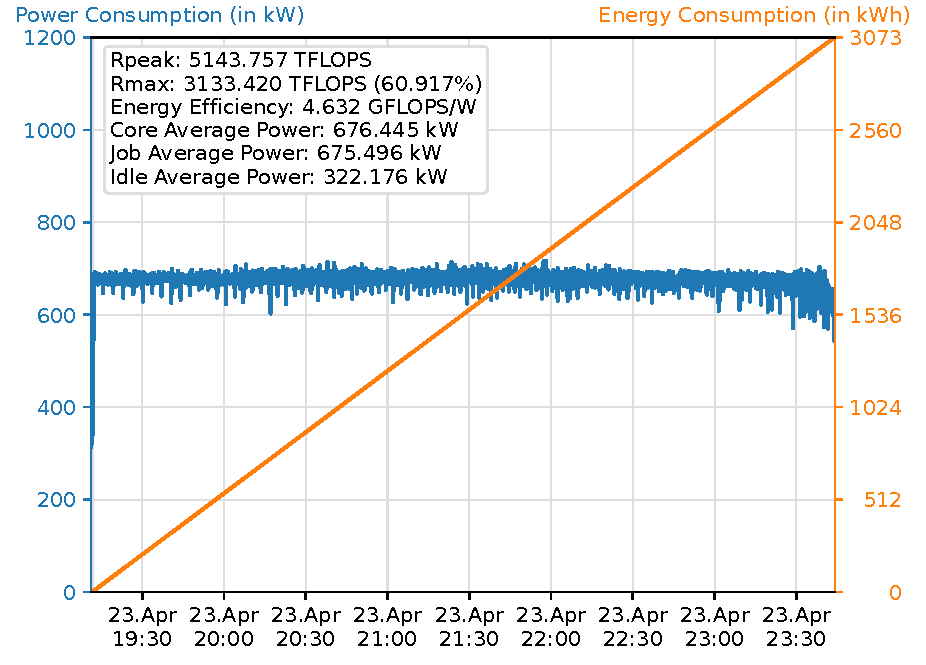
\includegraphics[width=\textwidth]{data/example-rwth-claix-2023/cpu/summary.pdf}
        \caption{CPU Segment}
        \label{fig:example-rwth-claix-2023-cpu-summary}
    \end{subfigure}
    \hfill
    \begin{subfigure}{0.45\textwidth}
        \centering
        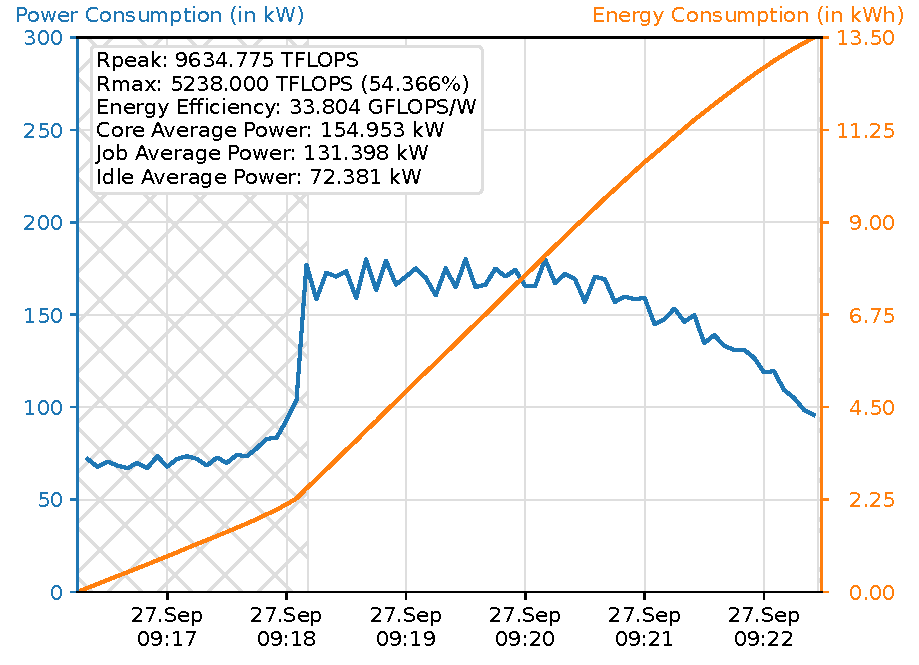
\includegraphics[width=\textwidth]{data/example-rwth-claix-2023/gpu/summary.pdf}
        \caption{GPU Segment}
        \label{fig:example-rwth-claix-2023-gpu-summary}
    \end{subfigure}
    \hfill
    \caption{Summary of the CLAIX-2023 Green500 submissions. Data from all measurement devices was resampled to a common \SI{5}{\second} interval. The hatched area indicates job execution outside the HPL core phase.}
    \label{fig:example-rwth-claix-2023-summary}
\end{figure}
